\documentclass{article}
\usepackage[margin=1in]{geometry}
\usepackage{amsmath}
\usepackage{amssymb}
\usepackage{amsthm}
\usepackage{verbatim}
\usepackage{multicol}
\usepackage[inline]{asymptote}
\usepackage{commath}
\usepackage{color} % colors and color names
\usepackage[font=it]{caption}
\usepackage{siunitx}
\usepackage{hyperref}
% character encodings
\usepackage[utf8]{inputenc}
\usepackage{float}

\begin{document}
\begin{center}
  {\LARGE \textbf{Analysis of period-mass Dependence of Momentum Induced Pursuit Curves Using Advanced Numeric Techniques}}\\[.1in]
  \large{\textit{Siena Guerrero, Jonathan Hayase, Tyler Sam, Ricky Shapley}}\\[0.2em]
  \normalsize
    Harvey Mudd College, 28 April 2017\\
    Project GitHub: \url{https://github.com/PythonNut/sipz}
\end{center}

\begin{multicols}{2}
  \section{Introduction}
  In this project, we decided to study pursuit curves with momentum and model them with differential equations. In particular, we set out to determine what the pursuit curve of a predator chasing after a prey moving in sinusoidal motion would look like. In order to make this situation more entertaining, we decided to make our predator Prof Kozai and our prey a wind-up mouse toy. The specific scene we created is as follows:

  Professor Kozai was sitting in his office one day, winding up his favorite wind-up mouse toy that moves in sinusoidal waves. Unfortunately, the mouse fell out of Prof. Kozai’s hands and onto his desk, it ran out of Prof. Kozai’s office with a page of the Math 45 Final Exam. Panicking over the loss of one of his exam sheets, Prof. Kozai ran out of his office in pursuit of the mouse.

  \section{Project Goals}
  Our goal was to find out whether the predator would catch the prey, and if so, at what time was the prey caught.

  \section{Differential Model}
  To model this scenario, we ended up using two equations, both of which have time as the independent variable. $\vec p$ is the position of the mouse in two dimensions, and $\vec k$ is the position of Prof. Kozai in two dimensions.

  To create differential equations that model this scenario, we made the assumption that the mouse travels in perfect sinusoidal motion, and that Professor Kozai has momentum, has no speed limit, and will always accelerate towards the mouse.

  The resulting differential equations are:

  \begin{align*}
    \dod{\vec p}{t} &= \hat{\mathbf{i}} + A \sin \omega t\\
    \dod[2]{\vec k}{t} &= \frac{\vec p - \vec k}{m \norm{\vec p - \vec k}}
  \end{align*}

  The first differential equation models the mouse’s sinusoidal motion. It travels in the x direction with constant velocity, and its y position varies as a sine wave with time.
  The second differential equation models Professor Kozai’s motion. The equation imitates the form of a typical pursuit curve differential equation, but Prof. Kozai accelerates toward the mouse instead of simply moving in that direction. The mass term on the bottom of the fraction arises from solving the force equation for Prof. Kozai’s motion, and the rest of the expression is simply the unit vector that points at the prey.

  \section{Solution}
  Since this is a second order system of differential equations, we are currently unable to solve it analytically.

  We researched many methods of solving differential equations numerically, and of the twenty algorithms we tested, Verner's "Most Efficient" 9/8 Runge-Kutta Method (9th Order Interpolant) was the only method capable of solving the DE to satisfactory accuracy at an acceptable speed. Most other methods were either too slow, or accumulated numerical errors which destroyed the periodic behavior of the solution.

  We plotted our solution and got solutions of the following form, which shows how Prof. Kozai moves through space:

  \begin{figure}[H]
    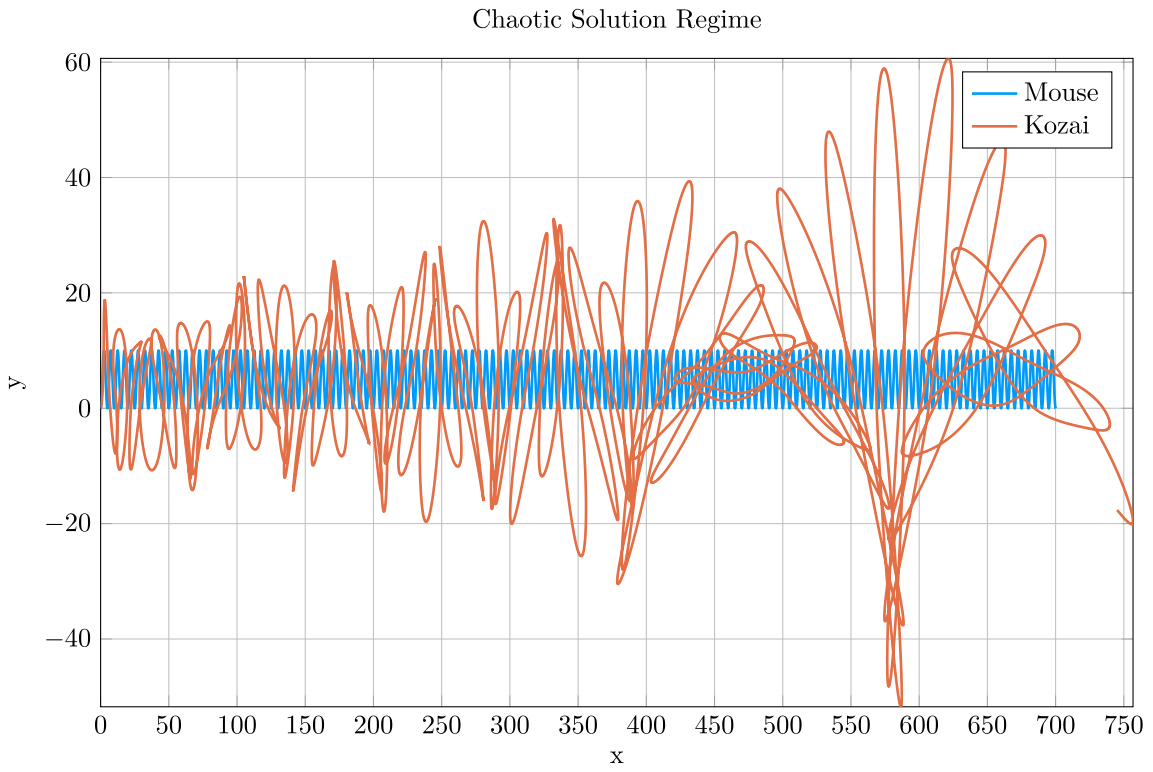
\includegraphics[scale=0.2]{chaotic}
    \caption{Initial chaotic solution regime}
  \end{figure}

  We quickly realized that this solution exhibited chaotic motion that was extremely difficult to analyze. To make the solution more approachable, we increased Professor Kozai’s mass to minimize the chaos. After doing so, we got solutions that looked like:

  \begin{figure}[H]
    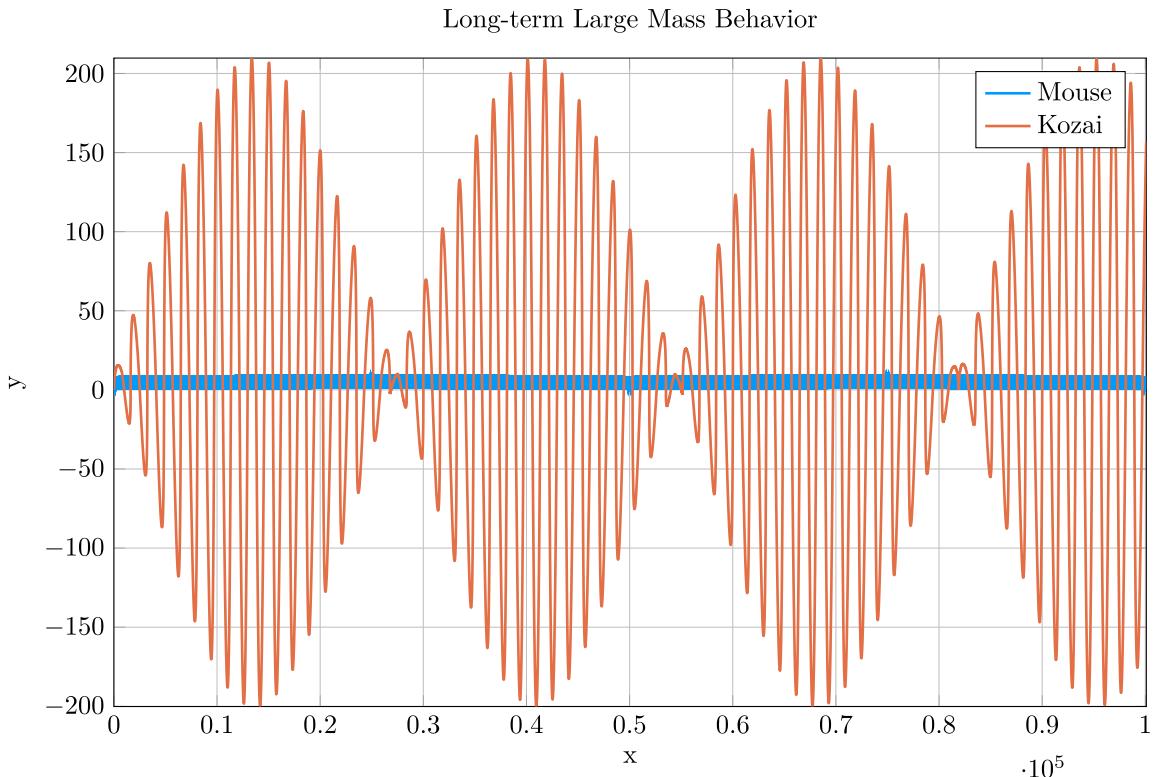
\includegraphics[scale=0.2]{longterm}
    \caption{Stable, periodic solution regime}
  \end{figure}

  We noticed that Professor Kozai ended up over $200$ units away from the $x$ axis in the $y$ direction when the mouse oscillated between $10$ and $-10$. This occurs because of constructive and deconstructive interference. Professor Kozai picks up momentum if he intersects with the mouse and is moving in the same direction since he spends longer accelerating in that direction. He loses momentum if he intersects with the mass and is moving in the opposite direction because he will begin accelerating in the opposite direction sooner. Since the phase of the mouse doesn’t perfectly align with Prof. Kozai’s natural oscillation frequency, Prof. Kozai will shift in and out of phase with the mouse, and hence experience both constructive and destructive interference.

  \section{Fourier Transforms}
  The curve clearly has a large period envelope function, created by much higher frequency oscillations. We used a Fourier Transform determine the both of these frequencies. We got the following results:


  \begin{figure}[H]
    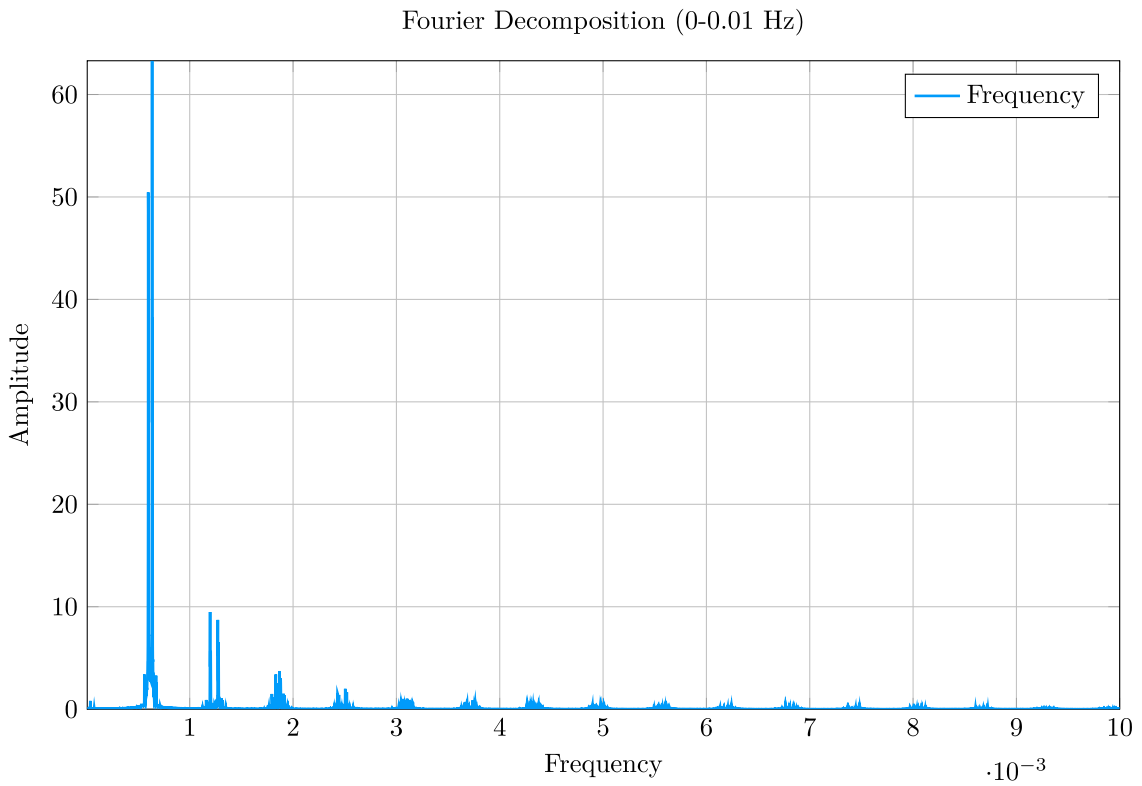
\includegraphics[scale=0.2]{fourier_high}
    \caption{Fourier transform of data from Figure 2}
  \end{figure}

  We can see that the frequency of the short-term period is approximately $\SI{3.8e-5}{\hertz}$.

  Focusing on very low frequency signals yielded the following:

  \begin{figure}[H]
    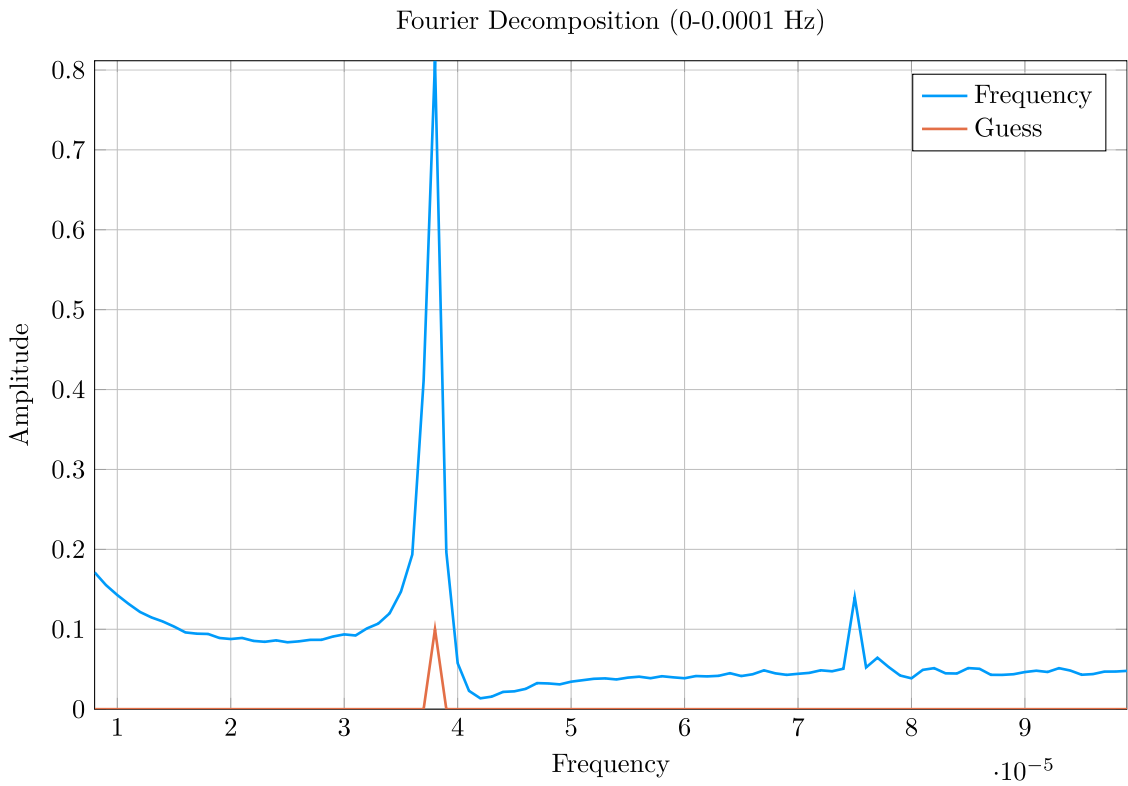
\includegraphics[scale=0.2]{fourier_low}
    \caption{Closeup of data from $0$ - $\SI{0.001}{\hertz}$}
  \end{figure}

  \section{Additional Observations}

  After finding the frequencies at one mass, we considered how changing the mass affects the period of both oscillatory frequencies. To do this, we wrote a distributed system to solve large numbers of related IVPs in parallel and performed the Fourier Transforms on the resulting solutions. Then, using Julia to fit a curve to the functions, we determined that the small period was linear with mass, and the large period was quadratic. Or in other words, the period of the fast oscillation is directly proportional to Prof. Kozai’s mass, and the period of the envelope function is proportional to the square of Prof. Kozai’s mass. Shown are plots of both periods as a function of Kozai's mass:
  \begin{figure}[H]
    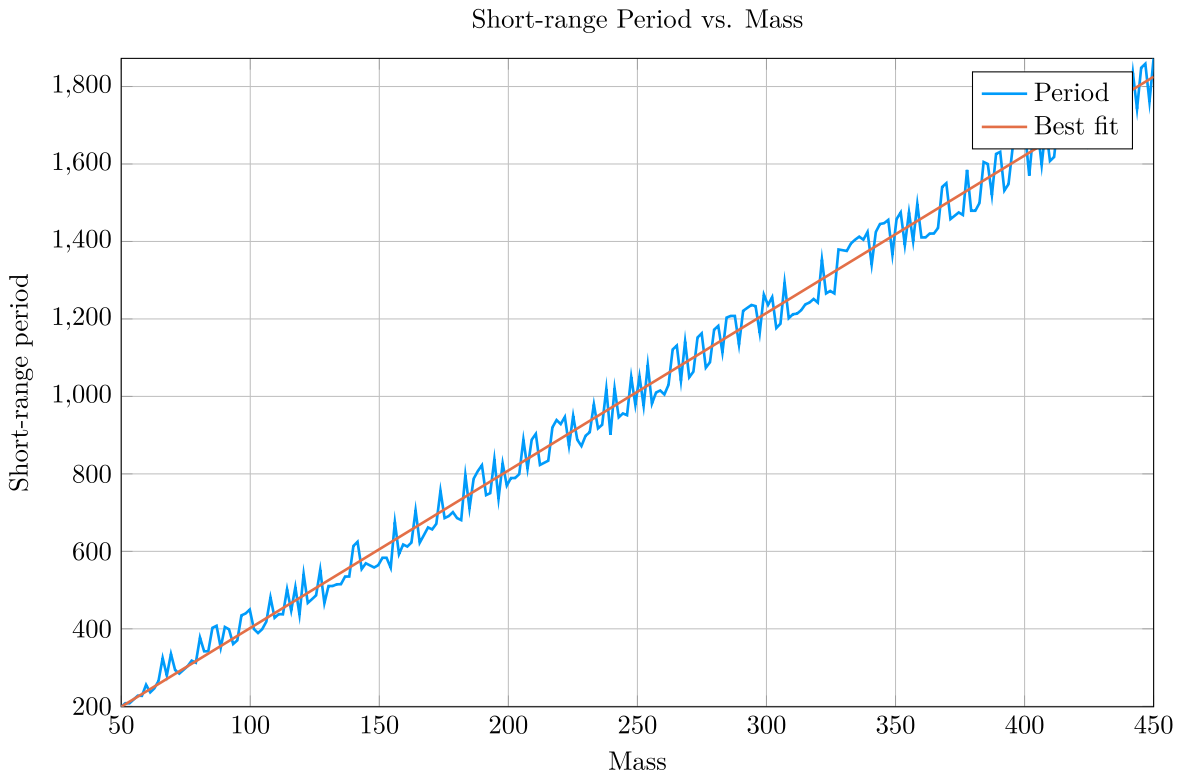
\includegraphics[scale=0.2]{short_period}
    \caption{95\% confidence interval for short-period oscillations is $T = (-4 \pm 10) + (10.42 \pm 0.03)m$}
  \end{figure}

  \begin{figure}[H]
    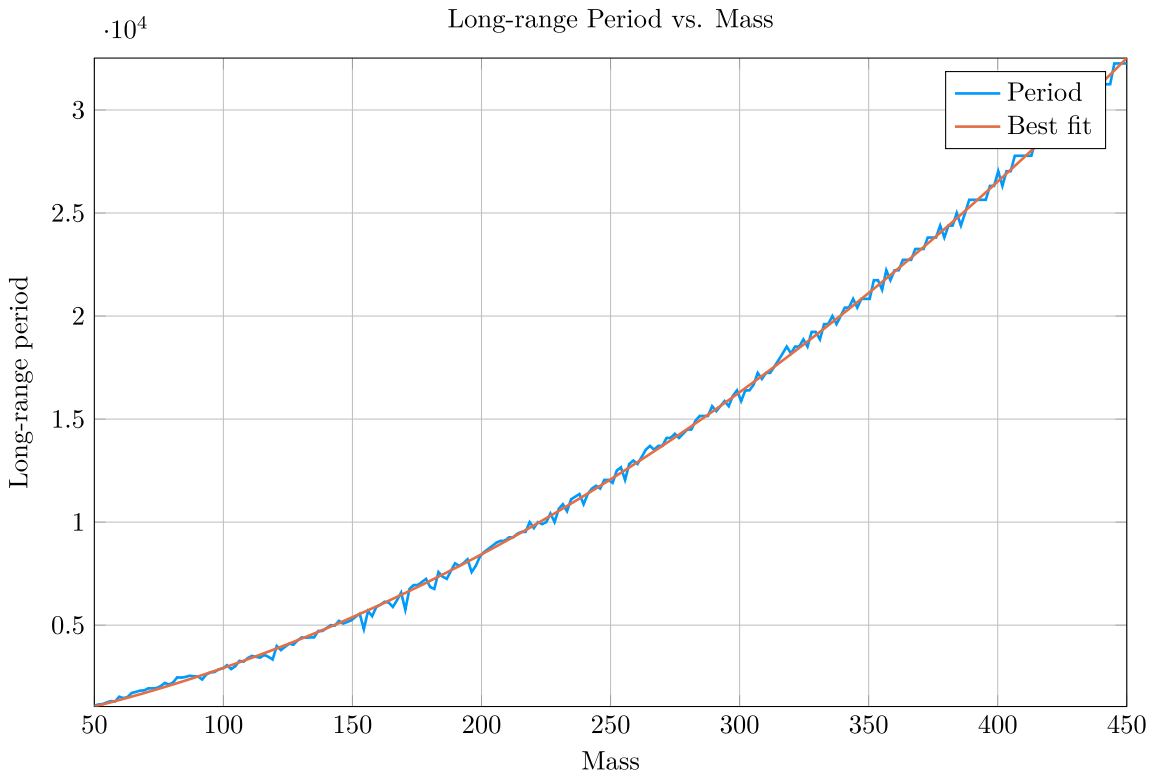
\includegraphics[scale=0.2]{long_period}
    \caption{95\% confidence interval for long-period oscillations is $T = (-200 \pm 100) + (19.8 \pm 0.9)m + (0.118 \pm 0.002)m^2$}
  \end{figure}

  \section{Discussion}
  We concluded that Prof. Kozai will never catch the mouse in a momentum based system where his mass is large. Although he gets close at points, in our numerical model, he will always lag slightly behind the mouse, even when his y coordinate is small. We can intuitively justify this by realizing that due to his large mass, he will be unable to change direction as quickly as the sine curve, so the mouse will continuously evade him.
  The instances where Prof. Kozai remains close to the mouse are at the nodes of the envelope function. These are also the times when he is traveling the slowest as he oscillates near the mouse. We can calculate when these instances occur using the relationship that the period of these nodes is proportional to the square of Prof. Kozai’s mass.

  \section{References}
  \begin{enumerate}
  \item \url{http://mathworld.wolfram.com/Runge-KuttaMethod.html}
  \item \url{http://docs.juliadiffeq.org/latest/}
  \item \url{http://people.math.sfu.ca/~jverner/RKV98.IIa.Efficient.000000349.081209.FLOAT6040OnWeb}
  \end{enumerate}
\end{multicols}
\end{document}
